\documentclass[sigconf,nonacm]{acmart}

\usepackage{booktabs}
\usepackage{multirow}
\usepackage{graphicx}
\usepackage{subcaption}
\usepackage{amsmath}
\usepackage{microtype}
\usepackage{enumitem}

\setlist{nosep, leftmargin=1.4em, topsep=2pt}

% Clean, balanced spacing for exact 6-page ACM SIGCONF layout
\setlength{\textfloatsep}{5pt plus 1.5pt minus 1.5pt}
\setlength{\floatsep}{4pt plus 1.5pt minus 1.5pt}
\setlength{\dbltextfloatsep}{5pt plus 1.5pt minus 1.5pt}
\setlength{\dblfloatsep}{4pt plus 1.5pt minus 1.5pt}
\setlength{\abovecaptionskip}{3pt}
\setlength{\belowcaptionskip}{1pt}

\begin{document}

\title[Transfer Learning vs.\ Scratch under Limited Data]{Transfer Learning vs.\ Training from Scratch under Limited Labeled Data}

\author{DSAA 5020 Final Project (Topic 8)}
\affiliation{%
  \institution{Data Science and Analytics Thrust, Fall 2026}
  \city{}
  \country{}
}

\begin{abstract}
Deep convolutional neural networks achieve strong visual recognition when trained on massive labeled corpora, yet acquiring fine-grained annotations in real-world domains is costly. In this study, we systematically investigate whether transfer learning from ImageNet-1K outperforms training from scratch under scarce labeled data on the 37-class Oxford-IIIT Pet dataset. Using ResNet-18 as our primary lightweight backbone across 44 controlled GPU runs (3 random seeds on primary conditions, nested stratified subsets spanning 5\%--100\% of training data, plus cross-backbone validation on MobileNetV3-Small), we compare four training regimes: random initialization (\emph{Scratch}), frozen linear probing (\emph{Frozen}), partial fine-tuning of the final stage (\emph{Partial FT}), and full network fine-tuning (\emph{Full FT}). Our results reveal four central findings. First, with only 10\% labeled data ($\sim$8 images/class), \emph{Frozen} achieves 83.65\% test accuracy (83.37\% Macro-F1) while updating only 0.17\% of parameters (19K) in 51s---outperforming \emph{Scratch} (14.09\% accuracy, +82.5\% train--validation gap) by +69.6 percentage points and $2.7\times$ faster training. Second, in low-data regimes (5\%--25\%), \emph{Frozen} consistently beats both \emph{Partial FT} and \emph{Full FT} (+5.8 to +12.7 pp), because updating millions of backbone weights on tiny subsets distorts pretrained representations and inflates overfitting; a crossover occurs around 50\% data, with \emph{Full FT} winning at 100\% (89.54\%). Third, just 5\% labeled data with \emph{Frozen} (81.55\%, 32.6s) outperforms 100\% \emph{Scratch} (55.95\%, 1250s) by +25.6 pp using $20\times$ fewer labels and $38\times$ less compute. Fourth, species-level error decomposition uncovers a sharp source-domain asymmetry: at 100\% data, dog breeds (well represented in ImageNet-1K) saturate under \emph{Frozen} (91.36\% vs.\ 91.27\% \emph{Full FT}), whereas 100\% of \emph{Full FT}'s gain comes from under-represented cat breeds (+2.74 pp).
\end{abstract}

\keywords{Transfer Learning, Fine-Tuning, Feature Extraction, Data Efficiency, Generalization Gap, Fine-Grained Classification}

\maketitle

\section{Introduction}
Training deep neural networks from random initialization typically requires tens of thousands of labeled examples to learn hierarchical visual features without memorizing training noise~\cite{deng2009imagenet,he2016deep}. In many practical data science applications---ranging from specialized wildlife monitoring to medical screening---labeled data are scarce, expensive, or slow to curate. Transfer learning addresses this bottleneck by reusing representations pretrained on large-scale benchmarks such as ImageNet-1K~\cite{russakovsky2015imagenet} and adapting them to downstream tasks via frozen feature extraction (linear probing) or partial/full fine-tuning~\cite{yosinski2014transferable,kornblith2019better}.

However, transferring pretrained representations is not a one-size-fits-all recipe. Prior theoretical and empirical studies show that unfreezing all layers on small downstream datasets can distort well-structured pretrained features and hurt generalization~\cite{kumar2022finetuning}, whereas keeping representations completely frozen may cap accuracy when labeled data grow or when downstream classes diverge from the pretraining label space~\cite{raghu2019transfusion}. Practitioners therefore face a concrete three-way trade-off across \emph{classification performance}, \emph{labeled data efficiency}, and \emph{computational cost}.

In this project, we conduct a controlled empirical study on the fine-grained \textbf{Oxford-IIIT Pet} dataset~\cite{parkhi2012cats} (37 cat and dog breeds) using \textbf{ResNet-18}~\cite{he2016deep} as our primary lightweight backbone, supplemented by \textbf{MobileNetV3-Small}~\cite{howard2019searching} for cross-architecture validation. We answer four research questions aligned with the project requirements:
\begin{enumerate}
  \item \textbf{Model Strategy under Scarce Labels (RQ1):} On a 10\% labeled subset ($\sim$8 images/class), how do training from scratch, frozen feature extraction, partial fine-tuning, and full fine-tuning compare in test accuracy and Macro-F1?
  \item \textbf{Data Efficiency Scaling (RQ2):} How much does scaling labeled data by $10\times$ (10\% $\to$ 100\%) improve frozen feature extraction, and where does the crossover between frozen extraction and fine-tuning emerge across 5\%--100\% data?
  \item \textbf{Generalization \& Representations (RQ3):} How do training--validation learning curves, generalization gaps, and penultimate-layer t-SNE embeddings explain overfitting and the benefit of pretrained representations?
  \item \textbf{Efficiency Trade-offs \& Error Modes (RQ4):} What is the Pareto frontier linking accuracy, labeled data volume, and GPU training time, and how does source--target domain overlap shape fine-grained breed errors?
\end{enumerate}

\section{Data Preparation and Experimental Protocol}

\subsection{Dataset Analysis and Leak-Free Splitting}
The Oxford-IIIT Pet dataset~\cite{parkhi2012cats} comprises 7,349 real-world pet photographs spanning \textbf{37 fine-grained breeds}: 12 cat breeds and 25 dog breeds, exhibiting wide pose, lighting, scale, and background variation. Officially, the dataset provides a \texttt{trainval} split (3,680 images) and a held-out \texttt{test} split (3,669 images).

\begin{figure*}[t]
  \centering
  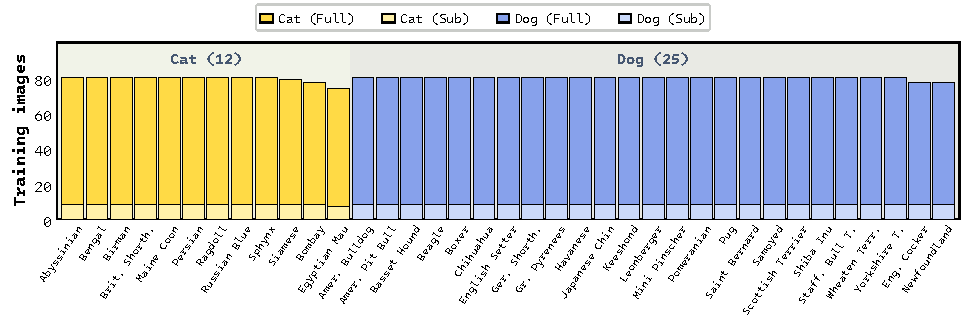
\includegraphics[width=0.92\textwidth]{figures/fig1_eda_class_distribution.pdf}
  \Description{Bar chart showing per-breed training sample counts across 37 pet breeds (12 cat breeds in yellow and 25 dog breeds in blue) for the 100\% pool and 10\% subset.}
  \caption{Exploratory data analysis of Oxford-IIIT Pet: per-breed training sample counts across 12 cat breeds (yellow) and 25 dog breeds (blue) for the 100\% training pool (74--80 images/class) and nested 10\% subset (7--8 images/class). The leak-free split totals 2,944 \texttt{Train (100\%)} (295 for 10\%), 736 fixed \texttt{Val}, and 3,669 official \texttt{Test} images.}
  \label{fig:eda}
\end{figure*}

To evaluate generalization cleanly without leaking test information into model selection or early stopping, we perform a deterministic stratified 80\%/20\% split of official \texttt{trainval} (fixed split seed 42) into:
\begin{itemize}
  \item \textbf{Full Training Pool (\texttt{Train 100\%}):} 2,944 images (74--80 per class, median 80).
  \item \textbf{Fixed Validation Set (\texttt{Val}):} 736 images (19--20 per class, median 20), shared identically across every run.
  \item \textbf{Held-Out Test Set (\texttt{Test}):} all 3,669 official test images (88--100 per class, median 100), locked until final evaluation.
\end{itemize}

From \texttt{Train 100\%}, we construct \textbf{strictly nested stratified subsets} for each seed $s \in \{42, 123, 2026\}$ by permuting each breed's pool indices with a seed-specific generator and retaining fraction $f$ (at least one image) per breed. For any fixed seed, the subsets satisfy $\mathcal{D}_{5\%} \subset \mathcal{D}_{10\%} \subset \mathcal{D}_{25\%} \subset \mathcal{D}_{50\%} \subset \mathcal{D}_{100\%}$ strictly, guaranteeing all 37 breeds appear even at 5\% (148 images, 4/class) and 10\% (295 images, 7--8/class), while varying $s$ honestly captures both small-sample subset variance and optimization variance. Figure~\ref{fig:eda} confirms balanced class coverage, with only minor dips in \emph{Egyptian Mau} (74 train images) and \emph{Bombay} (77).

\subsection{Backbones, Adaptation Strategies, and Training Protocol}
Our primary architecture is \textbf{ResNet-18}~\cite{he2016deep} (11.20M parameters, 512-dim penultimate feature), initialized either randomly (\emph{Scratch}) or with ImageNet-1K pretrained weights. To verify generality beyond one architecture, we replicate all 10\% and 100\% strategies on \textbf{MobileNetV3-Small}~\cite{howard2019searching} (1.56M parameters). We evaluate four strategies:
\begin{enumerate}
  \item \textbf{From Scratch (\emph{Scratch}):} Random initialization; all layers trainable (11.20M params on ResNet-18).
  \item \textbf{Frozen Feature Extraction (\emph{Frozen}):} Pretrained backbone frozen; only the 37-way linear head \texttt{fc} is trained (19.0K params, 0.17\% of ResNet-18).
  \item \textbf{Partial Fine-Tuning (\emph{Partial FT}, extension):} Pretrained stem and stages 1--3 frozen; only the final residual stage (\texttt{layer4}) and \texttt{fc} are trainable (8.41M params, 75.1\%).
  \item \textbf{Full Fine-Tuning (\emph{Full FT}):} Pretrained initialization with all layers unfrozen (11.20M params, 100\%).
\end{enumerate}

\textbf{Critical BatchNorm Hygiene.} A subtle pitfall in PyTorch transfer learning is calling \texttt{model.train()} globally during frozen extraction, which still updates BatchNorm running statistics on tiny mini-batches and degrades pretrained features. In \emph{Frozen} and \emph{Partial FT}, we explicitly keep all frozen layers in \texttt{.eval()} mode while setting only trainable modules to \texttt{.train()}.

\textbf{Fair Optimization \& Timing.} Training images use uniform augmentation (random resized $224\times 224$ crops with scale $[0.75, 1.0]$, horizontal flips, mild color jitter of $0.2$, and ImageNet normalization); validation and test images use deterministic resize to 256 followed by a $224\times 224$ center crop. Because randomly initialized networks require more epochs and higher learning rates than fine-tuned backbones, we assign principled strategy-specific budgets (Table~\ref{tab:config}) with AdamW~\cite{loshchilov2019decoupled} (weight decay $10^{-4}$), Cosine Annealing~\cite{loshchilov2017sgdr}, and early stopping on validation Macro-F1 (restoring the best validation checkpoint for testing). All 44 runs ran on a single \textbf{NVIDIA L4 GPU} (PyTorch 2.14, CUDA 13.0) using automatic mixed precision (AMP) and explicit CUDA synchronization around each training epoch for accurate wall-clock timing.

\begin{table}[t]
  \centering
  \caption{Training configuration per strategy on ResNet-18. Batch size is 32 for $\le$25\% data and 64 for $\ge$50\% data.}
  \label{tab:config}
  \renewcommand{\arraystretch}{0.92}
  \resizebox{\columnwidth}{!}{%
  \begin{tabular}{lcccc}
    \toprule
    \textbf{Strategy} & \textbf{Trainable Params} & \textbf{Backbone / Head LR} & \textbf{Max Ep.} & \textbf{Patience} \\
    \midrule
    Scratch    & 11.20M (100\%)  & $1\times 10^{-3}$ / $1\times 10^{-3}$ & 80 & 20 \\
    Frozen     & 19.0K (0.17\%)  & 0 / $3\times 10^{-3}$                 & 40 & 12 \\
    Partial FT & 8.41M (75.1\%)  & $3\times 10^{-4}$ / $1\times 10^{-3}$ & 40 & 12 \\
    Full FT    & 11.20M (100\%)  & $1\times 10^{-4}$ / $1\times 10^{-3}$ & 40 & 12 \\
    \bottomrule
  \end{tabular}%
  }
\end{table}

\begin{table*}[t]
  \centering
  \caption{Quantitative comparison across all 44 controlled runs on NVIDIA L4 GPU. Primary 10\% and 100\% ResNet-18 conditions report $\text{mean} \pm \text{std}$ over 3 seeds (42, 123, 2026); curve points (5\%, 25\%, 50\%) and MobileNetV3-Small use seed 42. Gap denotes $\text{Train Acc} - \text{Val Acc}$ at the best validation epoch. Bold marks best Test Acc/F1 per data fraction.}
  \label{tab:main_results}
  \renewcommand{\arraystretch}{0.86}
  \setlength{\tabcolsep}{4.5pt}
  \resizebox{\textwidth}{!}{%
  \begin{tabular}{lc l c c c c c c c c}
    \toprule
    \textbf{Backbone} & \textbf{Data \%} & \textbf{Strategy} & \textbf{Seeds} & \textbf{Trainable} & \textbf{Test Acc (\%)} & \textbf{Test Macro-F1 (\%)} & \textbf{Train--Val Gap} & \textbf{Best Ep.} & \textbf{Time to Best (s)} & \textbf{Total Time (s)} \\
    \midrule
    ResNet-18 & 5\%  & Scratch    & 1 & 11.20M & 8.64  & 8.52  & +86.43\% & 34.0 & 31.8  & 50.7 \\
    ResNet-18 & 5\%  & Frozen     & 1 & 19.0K  & \textbf{81.55} & \textbf{81.47} & +17.53\% & 23.0 & 21.4  & 32.6 \\
    ResNet-18 & 5\%  & Partial FT & 1 & 8.41M  & 69.94 & 69.76 & +29.21\% & 12.0 & 11.3  & 22.6 \\
    ResNet-18 & 5\%  & Full FT    & 1 & 11.20M & 68.90 & 68.81 & +29.76\% & 9.0  & 8.6   & 19.9 \\
    \midrule
    ResNet-18 & 10\% & Scratch    & 3 & 11.20M & 14.09 $\pm$ 1.09 & 13.74 $\pm$ 1.01 & +82.50\% & 73.0 & 126.8 & 139.0 $\pm$ 3.0 \\
    ResNet-18 & 10\% & Frozen     & 3 & 19.0K  & \textbf{83.65 $\pm$ 0.39} & \textbf{83.37 $\pm$ 0.45} & \textbf{+12.68\%} & 18.7 & 31.8  & 51.0 $\pm$ 17.6 \\
    ResNet-18 & 10\% & Partial FT & 3 & 8.41M  & 77.09 $\pm$ 0.73 & 76.65 $\pm$ 0.91 & +18.84\% & 7.7  & 13.3  & 33.8 $\pm$ 3.0 \\
    ResNet-18 & 10\% & Full FT    & 3 & 11.20M & 77.81 $\pm$ 0.50 & 77.36 $\pm$ 0.65 & +18.37\% & 14.7 & 25.3  & 46.1 $\pm$ 10.9 \\
    \midrule
    ResNet-18 & 25\% & Scratch    & 1 & 11.20M & 25.76 & 25.23 & +71.06\% & 64.0 & 273.0 & 341.0 \\
    ResNet-18 & 25\% & Frozen     & 1 & 19.0K  & \textbf{87.68} & \textbf{87.42} & +9.51\%  & 15.0 & 64.3  & 114.6 \\
    ResNet-18 & 25\% & Partial FT & 1 & 8.41M  & 85.04 & 84.74 & +13.59\% & 11.0 & 47.3  & 97.9 \\
    ResNet-18 & 25\% & Full FT    & 1 & 11.20M & 85.28 & 85.02 & +11.68\% & 7.0  & 30.1  & 81.3 \\
    \midrule
    ResNet-18 & 50\% & Scratch    & 1 & 11.20M & 37.20 & 36.60 & +58.90\% & 67.0 & 572.3 & 683.6 \\
    ResNet-18 & 50\% & Frozen     & 1 & 19.0K  & 87.90 & 87.77 & +8.29\%  & 21.0 & 178.5 & 281.1 \\
    ResNet-18 & 50\% & Partial FT & 1 & 8.41M  & 88.12 & 87.95 & +8.83\%  & 9.0  & 77.8  & 181.1 \\
    ResNet-18 & 50\% & Full FT    & 1 & 11.20M & \textbf{88.17} & \textbf{88.00} & +8.15\%  & 15.0 & 127.8 & 229.7 \\
    \midrule
    ResNet-18 & 100\% & Scratch    & 3 & 11.20M & 55.95 $\pm$ 1.33 & 55.39 $\pm$ 1.48 & +37.06\% & 68.7 & 1071.6 & 1250.1 $\pm$ 8.0 \\
    ResNet-18 & 100\% & Frozen     & 3 & 19.0K  & 88.70 $\pm$ 0.18 & 88.58 $\pm$ 0.16 & \textbf{+6.00\%}  & 21.7 & 337.9  & 524.2 $\pm$ 105.2 \\
    ResNet-18 & 100\% & Partial FT & 3 & 8.41M  & 88.73 $\pm$ 0.23 & 88.57 $\pm$ 0.20 & +7.71\%  & 13.7 & 214.1  & 403.0 $\pm$ 48.4 \\
    ResNet-18 & 100\% & Full FT    & 3 & 11.20M & \textbf{89.54 $\pm$ 0.30} & \textbf{89.41 $\pm$ 0.31} & +7.02\%  & 21.3 & 336.7  & 524.8 $\pm$ 134.2 \\
    \midrule
    MobileNetV3-S & 10\%  & Scratch    & 1 & 1.56M & 2.73  & 0.14  & $-$0.68\% & 1.0  & 9.1   & 46.7 \\
    MobileNetV3-S & 10\%  & Frozen     & 1 & 0.63M & \textbf{75.14} & \textbf{74.87} & +22.28\% & 11.0 & 20.0  & 41.7 \\
    MobileNetV3-S & 10\%  & Partial FT & 1 & 1.27M & 66.61 & 66.09 & +26.22\% & 24.0 & 42.2  & 63.1 \\
    MobileNetV3-S & 10\%  & Full FT    & 1 & 1.56M & 65.44 & 64.59 & +27.45\% & 23.0 & 41.7  & 63.2 \\
    \midrule
    MobileNetV3-S & 100\% & Scratch    & 1 & 1.56M & 41.24 & 40.75 & +48.74\% & 59.0 & 969.8 & 1295.1 \\
    MobileNetV3-S & 100\% & Frozen     & 1 & 0.63M & \textbf{86.37} & \textbf{86.20} & +10.19\% & 31.0 & 494.8 & 635.1 \\
    MobileNetV3-S & 100\% & Partial FT & 1 & 1.27M & 82.94 & 82.74 & +10.05\% & 16.0 & 250.0 & 436.4 \\
    MobileNetV3-S & 100\% & Full FT    & 1 & 1.56M & 84.27 & 84.09 & +9.61\%  & 27.0 & 421.4 & 607.5 \\
    \bottomrule
  \end{tabular}%
  }
\end{table*}

\section{Model Comparison with Limited Data (RQ1)}
Table~\ref{tab:main_results} and Figure~\ref{fig:comp10} present the 3-seed comparison on the 10\% labeled subset (295 training images, $\sim$8 per breed). Two striking phenomena emerge:

\begin{figure}[t]
  \centering
  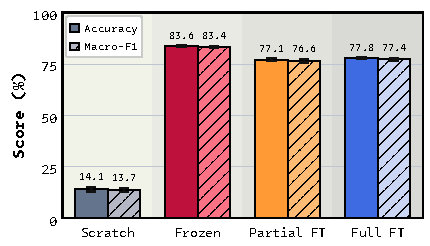
\includegraphics[width=0.86\columnwidth]{figures/fig2_model_comparison_10pct.pdf}
  \Description{Grouped bar chart comparing Test Accuracy and Macro-F1 of Scratch, Frozen, Partial FT, and Full FT on 10\% data.}
  \caption{ResNet-18 test accuracy and Macro-F1 on the 10\% labeled subset ($\text{mean} \pm \text{std}$, 3 seeds). Frozen feature extraction outperforms both random initialization (+69.6 pp) and full fine-tuning (+5.8 pp).}
  \label{fig:comp10}
\end{figure}

\textbf{1. Transfer Learning Overwhelms Random Initialization.} Training ResNet-18 from scratch on 295 images collapses to \textbf{14.09 $\pm$ 1.09\%} test accuracy (13.74\% Macro-F1)---barely above random chance ($2.7\%$) for 37 classes---despite training for 73 epochs and memorizing nearly 100\% of training images. By contrast, all three pretrained strategies jump above 77\% accuracy with tight cross-seed stability ($\text{std} < 1\%$), confirming that low- and mid-level visual hierarchies cannot be learned reliably from $\sim$8 samples per class.

\textbf{2. Frozen Extraction Beats Fine-Tuning under Scarce Labels.} Counter-intuitively, \emph{Frozen} (\textbf{83.65 $\pm$ 0.39\%} accuracy, 83.37\% Macro-F1) outperforms both \emph{Full FT} (77.81 $\pm$ 0.50\%, $-5.84$ pp) and \emph{Partial FT} (77.09 $\pm$ 0.73\%, $-6.56$ pp) across every seed. This mirrors the feature-distortion mechanism analyzed by Kumar et al.~\cite{kumar2022finetuning}: when a randomly initialized linear head emits large initial gradients on only 295 examples, backpropagating into 8.4M--11.2M backbone parameters warps well-calibrated ImageNet filters to fit small-sample idiosyncrasies. At 5\% data ($\sim$4 images/class), the margin widens to \textbf{+12.65 pp} (\emph{Frozen} 81.55\% vs.\ \emph{Full FT} 68.90\%). Keeping the backbone frozen acts as an implicit structural regularizer that preserves rich pretrained semantics while fitting only 19K linear weights.

\section{Data Efficiency Scaling (RQ2)}
To quantify how labeled data volume interacts with transfer strategy, Figure~\ref{fig:data_eff} plots the full 5\%--100\% data efficiency curve alongside the direct 10\% vs.\ 100\% comparison.

\textbf{Effect of $10\times$ More Data on Frozen Extraction.} Scaling labeled data tenfold from 10\% (295 images) to 100\% (2,944 images) lifts \emph{Frozen} ResNet-18 from \textbf{83.65\% $\to$ 88.70\%} test accuracy (+5.05 pp; Macro-F1 83.37\% $\to$ 88.58\%, +5.21 pp), while halving cross-seed variance ($\pm 0.39\% \to \pm 0.18\%$) and cutting the generalization gap from +12.68\% to +6.00\%. Crucially, marginal gains exhibit strong diminishing returns: moving from 5\% $\to$ 25\% ($5\times$ data) yields +6.13 pp (81.55\% $\to$ 87.68\%), whereas quadrupling data again from 25\% $\to$ 100\% adds only +1.02 pp (87.68\% $\to$ 88.70\%). Because a linear classifier over fixed 512-dim features has low capacity, $\sim$20 images per breed already estimates near-optimal separating hyperplanes.

\textbf{Crossover Between Frozen Extraction and Fine-Tuning.} Across the 5-point curve, \emph{Frozen} dominates in low-data regimes (5\%: +12.7 pp; 10\%: +5.8 pp; 25\%: +2.4 pp), but \textbf{a clean crossover emerges at 50\% data} (1,472 images, $\sim$40/class), where \emph{Full FT} (88.17\%) and \emph{Partial FT} (88.12\%) edge past \emph{Frozen} (87.90\%). At 100\% data, \emph{Full FT} reaches the overall peak of \textbf{89.54 $\pm$ 0.30\%} accuracy (89.41\% Macro-F1), surpassing \emph{Frozen} by +0.84 pp and \emph{Partial FT} by +0.81 pp.

\textbf{Extreme Data Efficiency vs.\ Training from Scratch.} Even with 100\% of training labels (2,944 images), \emph{Scratch} attains only \textbf{55.95 $\pm$ 1.33\%} accuracy---still trailing \textbf{5\% \emph{Frozen}} (81.55\%, 148 images) by \textbf{25.60 pp}. Thus, ImageNet pretraining delivers far stronger fine-grained recognition using \textbf{$20\times$ fewer labeled examples} than learning from scratch.

\begin{figure}[t]
  \centering
  \begin{subfigure}{\columnwidth}
    \centering
    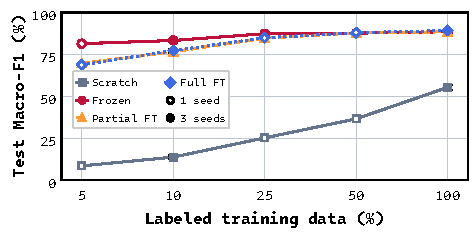
\includegraphics[width=0.95\columnwidth]{figures/fig3a_data_efficiency_curve.pdf}
    \caption{Test Macro-F1 across nested subsets (5\%--100\%).}
    \label{fig:data_eff_curve}
  \end{subfigure}
  \par\smallskip
  \begin{subfigure}{\columnwidth}
    \centering
    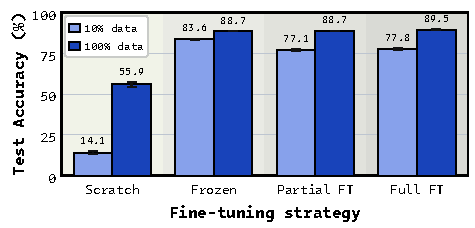
\includegraphics[width=0.95\columnwidth]{figures/fig3b_10_vs_100_accuracy.pdf}
    \caption{10\% vs.\ 100\% Test Accuracy (3-seed $\text{mean} \pm \text{std}$).}
    \label{fig:data_eff_bars}
  \end{subfigure}
  \Description{Top: line chart of Test Macro-F1 across 5\% to 100\% labeled data for four strategies. Bottom: grouped bar chart comparing 10\% vs 100\% Test Accuracy.}
  \caption{Data efficiency analysis on ResNet-18. (a) Filled markers indicate 3-seed runs and open markers indicate single-seed runs, illustrating the crossover between \emph{Frozen} and \emph{Full FT} at 50\% data and the persistent gap over \emph{Scratch}. (b) Direct 10\% vs.\ 100\% Test Accuracy comparison.}
  \label{fig:data_eff}
\end{figure}

\begin{figure}[t]
  \centering
  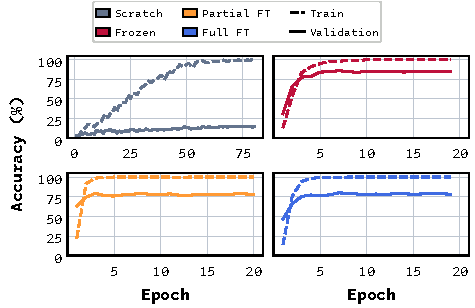
\includegraphics[width=0.95\columnwidth]{figures/fig4a_generalization_curves.pdf}
  \Description{2x2 grid of train vs validation accuracy curves across epochs for four strategies on 10\% data.}
  \caption{Training (dashed) vs.\ Validation (solid) accuracy trajectories on 10\% labeled data (ResNet-18, seed 42); shaded regions denote the generalization gap.}
  \label{fig:gen_curves}
\end{figure}

\begin{figure}[t]
  \centering
  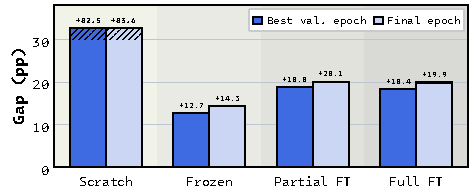
\includegraphics[width=0.95\columnwidth]{figures/fig4b_generalization_gap.pdf}
  \Description{Grouped bar chart of 3-seed mean Train-Val generalization gap at best validation and final epochs, with Scratch truncated at 30 pp.}
  \caption{3-seed mean Train--Val accuracy gap on 10\% labeled data (ResNet-18) at the best validation epoch and final epoch. Hatched \emph{Scratch} bars are truncated at 30\,pp with exact values annotated above.}
  \label{fig:gen_gap}
\end{figure}

\section{Generalization and Representation Analysis (RQ3)}

\subsection{Overfitting Dynamics and Generalization Gap}
Figures~\ref{fig:gen_curves} and~\ref{fig:gen_gap} contrast training and validation accuracy curves on the 10\% subset alongside the quantified generalization gap ($\text{Train Acc} - \text{Val Acc}$). \emph{Scratch} exhibits severe overfitting: training accuracy climbs to $\sim$99\% by epoch 60 while validation accuracy stalls below 16\%, opening an \textbf{+82.50\%} gap at the best validation epoch (+83.6\% at final epoch). Even at 100\% data, \emph{Scratch} retains a large +37.06\% gap (Table~\ref{tab:main_results}).

Pretrained models converge $4\times$--$10\times$ faster (peaking in 8--19 epochs vs.\ 73 for \emph{Scratch}) and sharply curb overfitting. Comparing the three transfer regimes on 10\% data clarifies why \emph{Frozen} wins: both \emph{Partial FT} and \emph{Full FT} saturate near $\sim$100\% training accuracy by epoch 3--5 and plateau around $\sim$79\% validation accuracy (best-epoch gaps of \textbf{+18.84\%} and \textbf{+18.37\%}), whereas \emph{Frozen} climbs smoothly to $\sim$86\% validation accuracy with the tightest generalization gap (\textbf{+12.68\%}). At 100\% data, larger supervision shrinks the gap across all transfer strategies to 6.0\%--7.7\%, enabling \emph{Full FT} to exploit its extra plasticity safely.

\begin{figure*}[t]
  \centering
  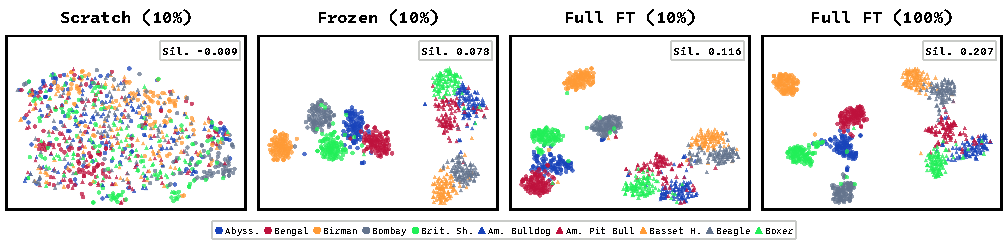
\includegraphics[width=0.96\textwidth]{figures/fig5_tsne_representations.pdf}
  \Description{Four side-by-side t-SNE scatter plots comparing penultimate test embeddings for Scratch 10\%, Frozen 10\%, Full FT 10\%, and Full FT 100\%.}
  \caption{t-SNE projections of 512-dimensional ResNet-18 penultimate features on the held-out test set (first 10 pet breeds for visual clarity), annotated with Euclidean Silhouette scores computed in the original 512-dim feature space.}
  \label{fig:tsne}
\end{figure*}

\subsection{Representation Geometry via t-SNE}
To inspect \emph{what} models learn beyond scalar metrics, Figure~\ref{fig:tsne} plots 2D t-SNE projections~\cite{vandermaaten2008tsne} of ResNet-18's 512-dim penultimate test embeddings (first 10 breeds) alongside high-dimensional Silhouette scores:
\begin{itemize}
  \item \textbf{Scratch (10\%):} Embeddings collapse into an unstructured cloud (Silhouette $-0.009$), confirming that 8 images/breed cannot induce class-discriminative filters.
  \item \textbf{Frozen Pretrained (10\%):} Without updating a single convolutional weight, ImageNet features partition breeds into crisp semantic clusters with Silhouette $0.078$.
  \item \textbf{Full FT (10\%) vs.\ Full FT (100\%):} At 10\% data, \emph{Full FT} yields slightly tighter local clusters (Silhouette $0.116$) yet lower 37-class accuracy (77.81\%) than \emph{Frozen} (83.65\%), showing that aggressive weight updates compact easy breeds while distorting margins for harder classes. At 100\% data, \emph{Full FT} achieves clean global separation (Silhouette $0.207$) and peak accuracy (89.54\%).
\end{itemize}

\section{Efficiency Trade-Offs and Fine-Grained Analysis (RQ4)}

\subsection{Performance--Data--Compute Pareto Trade-Off}
Figure~\ref{fig:tradeoff} maps Test Macro-F1 against total GPU training time (log scale) across 10\% and 100\% ResNet-18 runs, with the dashed Pareto frontier identifying non-dominated regimes. Together with Table~\ref{tab:main_results}, three operating regimes stand out:

\begin{figure}[t]
  \centering
  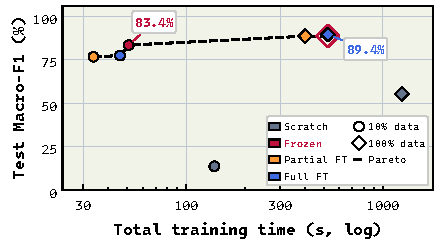
\includegraphics[width=0.88\columnwidth]{figures/fig6_efficiency_tradeoff.pdf}
  \Description{Scatter plot of Test Macro-F1 versus total GPU training time on a log scale with a dashed Pareto frontier across 10\% and 100\% data.}
  \caption{Pareto trade-off between Test Macro-F1, total L4 GPU training time (log scale), and labeled data budget on ResNet-18. \emph{Scratch} is strictly Pareto-dominated at both 10\% and 100\% data.}
  \label{fig:tradeoff}
\end{figure}

\begin{enumerate}
  \item \textbf{Strict Dominance over Scratch:} Both 10\% \emph{Scratch} (13.7\% F1, 139s) and 100\% \emph{Scratch} (55.4\% F1, 1250s) fall far below the frontier. At 100\% data, \emph{Scratch} burns $2.4\times$ more compute than \emph{Full FT} (525s) and $38\times$ more than 5\% \emph{Frozen} (32.6s) while trailing by 34.0 and 26.1 F1 points.
  \item \textbf{High-Efficiency Sweet Spot (\emph{Frozen 10\%}):} Using only 295 labeled images, 19K trainable params, 385 MB peak GPU memory (vs.\ 999 MB for \emph{Full FT 100\%}), and 31.8s to peak validation (51.0s total), \emph{Frozen (10\%)} achieves \textbf{83.4\% Macro-F1}---\textbf{93.2\%} of peak 100\% \emph{Full FT} performance at \textbf{10\% annotation cost} and \textbf{9.7\% training time}.
  \item \textbf{Maximum-Accuracy Regime (\emph{Full FT 100\%}):} Pushing from 83.4\% to \textbf{89.4\% Macro-F1} (+6.0 pp) requires $10\times$ more labels and $10.3\times$ more compute (525s). Meanwhile, \emph{Partial FT (100\%)} forms a strong Pareto compromise: it matches \emph{Frozen (100\%)} (88.6\% F1) while finishing 23\% faster (403s) and using half the peak GPU memory of \emph{Full FT} (515 MB vs.\ 999 MB).
\end{enumerate}

\subsection{Source-Domain Asymmetry and Error Analysis}
Dissecting Oxford-IIIT Pet errors by species uncovers a deeper mechanism governing transfer learning. ImageNet-1K~\cite{russakovsky2015imagenet} allocates roughly \textbf{120 classes to fine-grained dog breeds} (from Stanford Dogs), but only \textbf{$\sim$5 classes to domestic cats} (\emph{tabby}, \emph{tiger cat}, \emph{Persian}, \emph{Siamese}, \emph{Egyptian cat}). Table~\ref{tab:species} and Figures~\ref{fig:error_pairs}--\ref{fig:error_species} show how this source-domain imbalance shapes downstream adaptation:

\begin{table}[t]
  \centering
  \caption{Species-level mean class F1 (\%, 3-seed $\text{mean} \pm \text{std}$) on ResNet-18. High ImageNet dog-breed overlap produces a +15.3 pp advantage under 10\% \emph{Frozen}; at 100\% data, 100\% of \emph{Full FT}'s gain over \emph{Frozen} comes from cat breeds (+2.74 pp).}
  \label{tab:species}
  \renewcommand{\arraystretch}{0.9}
  \resizebox{\columnwidth}{!}{%
  \begin{tabular}{clccc}
    \toprule
    \textbf{Data} & \textbf{Strategy} & \textbf{Cat F1 (12 cls)} & \textbf{Dog F1 (25 cls)} & \textbf{Dog $-$ Cat} \\
    \midrule
    10\%  & Scratch    & 14.85 $\pm$ 0.39 & 13.20 $\pm$ 1.36 & $-$1.64 pp \\
    10\%  & Frozen     & \textbf{73.00 $\pm$ 2.84} & \textbf{88.35 $\pm$ 1.38} & +15.34 pp \\
    10\%  & Partial FT & 70.62 $\pm$ 1.73 & 79.54 $\pm$ 0.96 & +8.93 pp \\
    10\%  & Full FT    & 70.90 $\pm$ 1.02 & 80.45 $\pm$ 1.32 & +9.55 pp \\
    \midrule
    100\% & Scratch    & 57.00 $\pm$ 1.50 & 54.61 $\pm$ 1.59 & $-$2.39 pp \\
    100\% & Frozen     & 82.78 $\pm$ 0.42 & \textbf{91.36 $\pm$ 0.06} & +8.58 pp \\
    100\% & Partial FT & 85.01 $\pm$ 0.24 & 90.28 $\pm$ 0.28 & +5.27 pp \\
    100\% & Full FT    & \textbf{85.52 $\pm$ 0.62} & 91.27 $\pm$ 0.16 & +5.76 pp \\
    \bottomrule
  \end{tabular}%
  }
\end{table}

\begin{figure}[t]
  \centering
  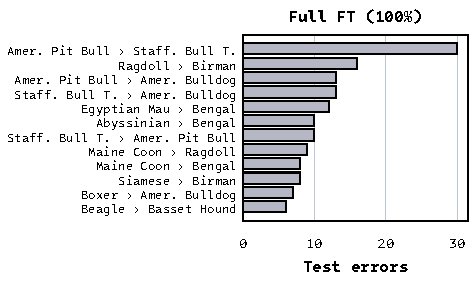
\includegraphics[width=0.95\columnwidth]{figures/fig7a_confusion_pairs.pdf}
  \Description{Horizontal bar chart of top-12 confused breed pairs for Full FT 100\%.}
  \caption{Top-12 most confused test breed pairs for \emph{Full FT (100\%, seed 42)} on ResNet-18 (371 errors out of 3,669 test images).}
  \label{fig:error_pairs}
\end{figure}

\begin{figure}[t]
  \centering
  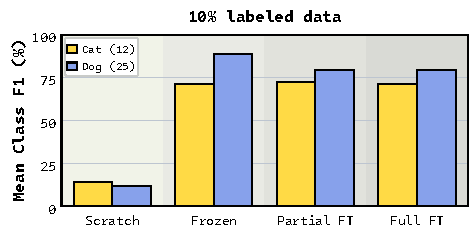
\includegraphics[width=0.95\columnwidth]{figures/fig7b_species_f1.pdf}
  \Description{Grouped bar chart comparing Cat vs Dog mean class F1 across strategies on 10\% data.}
  \caption{Cat (12 breeds) vs.\ Dog (25 breeds) mean class F1 on 10\% labeled data across training strategies (ResNet-18, seed 42).}
  \label{fig:error_species}
\end{figure}

\begin{itemize}
  \item \textbf{No Intrinsic Species Bias under Scratch:} Without pretraining, cat breeds are slightly \emph{easier} than dog breeds ($-1.64$ pp at 10\%, $-2.39$ pp at 100\%).
  \item \textbf{Sharp Dog Advantage under Frozen Pretraining:} Under 10\% \emph{Frozen}, dog breeds reach \textbf{88.35\%} F1 while cat breeds lag at \textbf{73.00\%} (\textbf{+15.34 pp} asymmetry). In 10\% \emph{Frozen} errors (616 total), 5 of the top 6 confused pairs are visually close cat breeds (\emph{Bengal $\to$ Egyptian Mau}: 39; \emph{British Shorthair $\leftrightarrow$ Russian Blue}: 59 combined; \emph{Ragdoll $\to$ Birman}: 20).
  \item \textbf{Where Full Fine-Tuning Actually Helps:} At 100\% data, dog breeds are already saturated by frozen ImageNet features (\emph{Frozen} 91.36\% vs.\ \emph{Full FT} 91.27\%, $-0.09$ pp). Conversely, unfreezing substantially boosts under-represented cat breeds (\textbf{+2.23 pp} \emph{Partial FT}, \textbf{+2.74 pp} \emph{Full FT}), explaining \textbf{virtually 100\% of \emph{Full FT}'s gain over \emph{Frozen}}. Residual errors under \emph{Full FT (100\%)} (Figure~\ref{fig:error_pairs}) reflect closely related morphotypes: \emph{American Pit Bull Terrier $\leftrightarrow$ Staffordshire Bull Terrier} (40 combined) and \emph{Ragdoll $\to$ Birman} (16).
\end{itemize}

\subsection{Cross-Backbone Validation}
To confirm generality beyond ResNet-18, Figure~\ref{fig:backbone} and Table~\ref{tab:main_results} evaluate \textbf{MobileNetV3-Small} ($7\times$ fewer parameters). Every qualitative finding replicates cleanly: on 10\% data, \emph{Scratch} collapses (2.73\% accuracy, 0.14\% Macro-F1), \emph{Frozen} leads at \textbf{75.14\%} (74.87\% Macro-F1), and unfreezing hurts (\emph{Partial FT} 66.61\%, \emph{Full FT} 65.44\%) with larger overfitting gaps (+26.2\%--27.5\% vs.\ +22.3\%). Notably, on this compact architecture, \emph{Frozen} retains a +2.1 pp edge even at 100\% data (86.37\% vs.\ 84.27\% \emph{Full FT}), confirming that lightweight inverted-residual networks are especially vulnerable to fine-tuning distortion.

\begin{figure}[t]
  \centering
  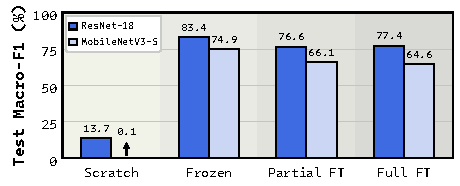
\includegraphics[width=0.92\columnwidth]{figures/fig8_backbone_comparison.pdf}
  \Description{Grouped bar chart comparing Test Macro-F1 of MobileNetV3-Small and ResNet-18 across four training strategies on 10\% data.}
  \caption{Cross-backbone validation on 10\% labeled data comparing ResNet-18 (11.2M params) and MobileNetV3-Small (1.56M params). Both architectures exhibit identical strategy rankings.}
  \label{fig:backbone}
\end{figure}

\section{Discussion, Limitations, and Conclusion}
\textbf{Domain-Similarity Caveat and Limitations.} Our experiments decisively confirm that transfer learning outperforms training from scratch with limited labeled data across accuracy, generalization, and compute. Two caveats merit attention. First, as our Cat-vs.-Dog analysis proves, the remarkable zero-adaptation accuracy of \emph{Frozen} features depends strongly on \textbf{source--target semantic overlap} with ImageNet-1K. In domains distant from natural imagery---such as histopathology, X-rays, or radar---frozen ImageNet features transfer less directly and require deeper fine-tuning~\cite{raghu2019transfusion}. Second, two-stage linear-probe-then-fine-tuning (\emph{LP-FT})~\cite{kumar2022finetuning} or stronger regularization (Mixup, RandAugment) could reduce \emph{Full FT}'s feature distortion at 10\% data and warrants future investigation.

\textbf{Actionable Takeaways.} Across 44 controlled GPU runs on Oxford-IIIT Pet, we derive three practical guidelines:
\begin{enumerate}
  \item \textbf{Never train from scratch} under scarce labels ($\le 80$ images/class) when a relevant pretrained backbone exists: even 5\% \emph{Frozen} beats 100\% \emph{Scratch} by +25.6 pp at $38\times$ lower compute.
  \item \textbf{Default to Frozen Feature Extraction} (keeping frozen BatchNorm layers in evaluation mode) when labeled data are scarce ($\le 25\%$, $\le 20$ images/class) or compute/memory is tight; it minimizes overfitting (+12.7\% gap) and beats full fine-tuning by +5.8--12.7 pp.
  \item \textbf{Switch to Full Fine-Tuning} once adequate labels are available ($\ge 50\%$, $\ge 40$ images/class), especially when target sub-domains (such as cat breeds here) are under-represented during pretraining.
\end{enumerate}

\bibliographystyle{ACM-Reference-Format}
\bibliography{references}

\end{document}
